\documentclass[border=10pt]{standalone}
\usepackage{tikz}
\usepackage{tikz-3dplot}
\usepackage{pgfplots}
\pgfplotsset{compat=1.18}
\usepackage{helvet}
\renewcommand{\familydefault}{\sfdefault}

\definecolor{emeraldpine}{HTML}{1A4D3E}
\definecolor{harvardcrimson}{HTML}{A51C30}
\definecolor{ethdarkblue}{HTML}{1F407A}
\definecolor{ethpetrol}{HTML}{007A87}
\definecolor{ethbronze}{HTML}{B87333}
\definecolor{ink}{HTML}{1A202C}
\definecolor{cardbg}{HTML}{F8FAFC}

\begin{document}
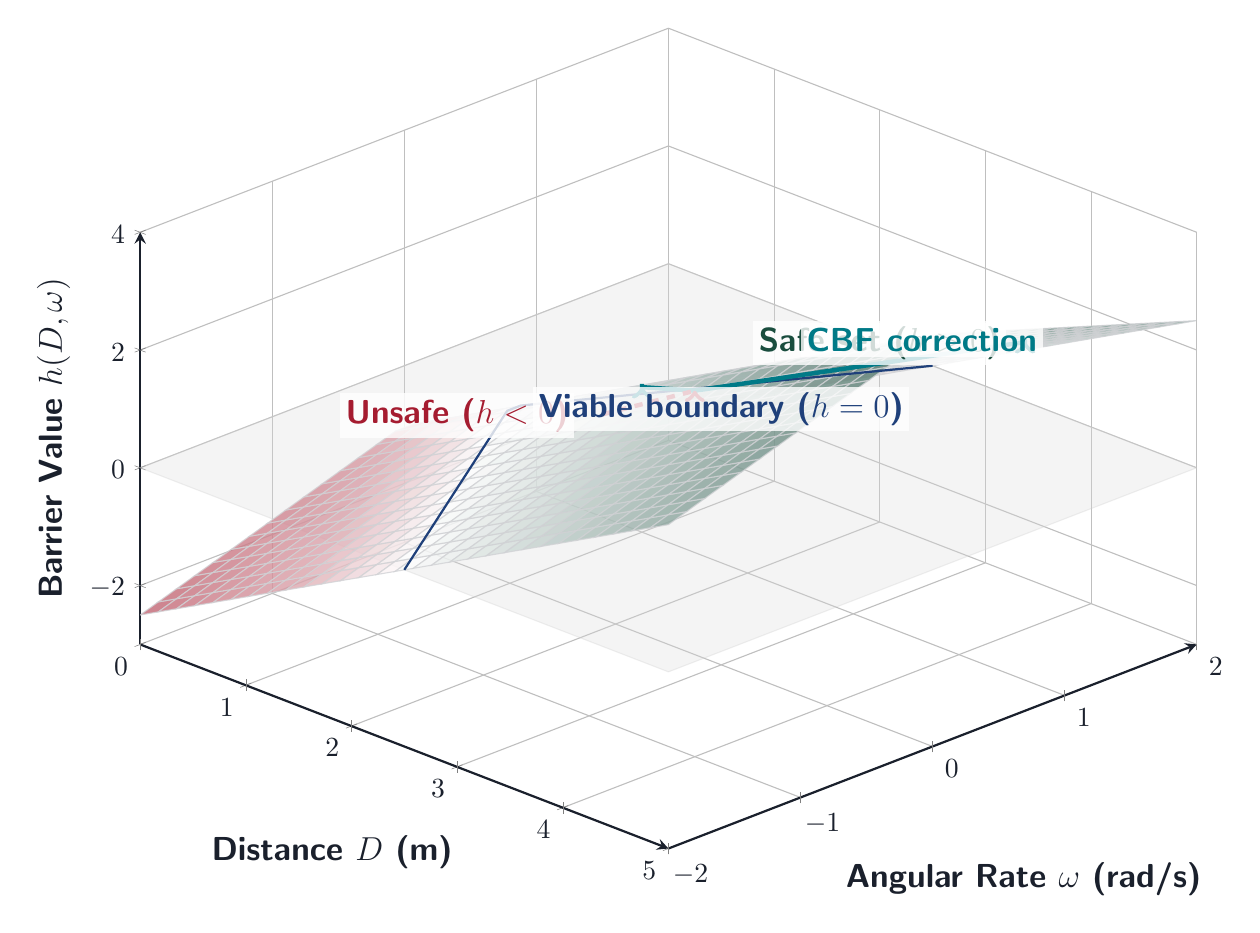
\begin{tikzpicture}
    \begin{axis}[
        width=15cm, height=12cm,
        view={45}{35},
        xlabel={Distance $D$ (m)},
        ylabel={Angular Rate $\omega$ (rad/s)},
        zlabel={Barrier Value $h(D, \omega)$},
        xmin=0, xmax=5,
        ymin=-2, ymax=2,
        zmin=-3, zmax=4,
        grid=major,
        colormap={cbfmap}{
            color=(harvardcrimson!80)
            color=(harvardcrimson!60)
            color=(harvardcrimson!40)
            color=(white)
            color=(emeraldpine!20)
            color=(emeraldpine!40)
            color=(emeraldpine!60)
            color=(emeraldpine!80)
        },
        point meta min=-3, point meta max=4,
        xlabel style={font=\large\bfseries, text=ink},
        ylabel style={font=\large\bfseries, text=ink},
        zlabel style={font=\large\bfseries, text=ink},
        ticklabel style={font=\normalsize, text=ink},
        axis lines=left,
        axis line style={thick, ink},
        z buffer=sort
    ]
    
    % The z=0 critical boundary plane
    \addplot3[
        surf,
        domain=0:5,
        domain y=-2:2,
        samples=2,
        opacity=0.3,
        fill=gray!30,
        draw=none,
    ] {0};
    
    % The CBF surface: h = D - 1 - 0.75*|omega|
    \addplot3[
        surf,
        domain=0:5,
        domain y=-2:2,
        samples=30,
        samples y=30,
        opacity=0.8,
        faceted color=ink!20!white,
    ] {x - 1 - 0.75*abs(y)};
    
    % Boundary curve h=0 -> D = 1 + 0.75*|omega|
    \addplot3[
        domain=-2:2,
        samples=40,
        thick,
        color=ethdarkblue,
    ] ( {1 + 0.75*abs(x)}, {x}, {0} );

    % Trajectory 1: Safe correction
    % Starts at D=4, omega=1.5, goes towards boundary, gets deflected
    \addplot3[
        domain=0:1,
        samples=20,
        ultra thick,
        ethpetrol,
        ->
    ] ( 
        {4 - 2.5*x}, 
        {1.5 - 0.5*x}, 
        {(4 - 2.5*x) - 1 - 0.75*abs(1.5 - 0.5*x)}
    );
    \addplot3[
        domain=0:1,
        samples=20,
        ultra thick,
        ethpetrol,
        ->
    ] ( 
        {1.5 + 0.5*x}, 
        {1.0 - 0.8*x}, 
        {(1.5 + 0.5*x) - 1 - 0.75*abs(1.0 - 0.8*x)}
    );
    
    % Trajectory 2: Uncorrected crossing
    \addplot3[
        domain=0:1,
        samples=20,
        ultra thick,
        dashed,
        harvardcrimson,
        ->
    ] (
        {1.5 - 1.5*x},
        {1.0 + 0.5*x},
        {(1.5 - 1.5*x) - 1 - 0.75*abs(1.0 + 0.5*x)}
    );

    % Labels
    \node[emeraldpine, font=\large\bfseries, fill=white, fill opacity=0.8, text opacity=1, inner sep=2pt] at (axis cs:4.5, 0, 3.5) {Safe set ($h > 0$)};
    \node[harvardcrimson, font=\large\bfseries, fill=white, fill opacity=0.8, text opacity=1, inner sep=2pt] at (axis cs:0.5, 0, -0.5) {Unsafe ($h < 0$)};
    \node[ethdarkblue, font=\large\bfseries, fill=white, fill opacity=0.8, text opacity=1, inner sep=2pt, anchor=north] at (axis cs:1.75, 1, 0) {Viable boundary ($h = 0$)};
    
    % Annotation for CBF correction
    \node[ethpetrol, font=\large\bfseries, fill=white, fill opacity=0.8, text opacity=1, inner sep=2pt, anchor=south west] at (axis cs:2.5, 1, 1) {CBF correction};

    \end{axis}
\end{tikzpicture}
\end{document}
